\documentclass[11pt]{article}
\usepackage[margin=1in]{geometry}
\usepackage{booktabs}
\usepackage{array}
\usepackage{graphicx}
\usepackage{pgfplots}
\usepackage{amsmath}
\pgfplotsset{compat=1.18}

\begin{document}

\begin{titlepage}
    \centering
    \vspace*{0.18\textheight}
    {\LARGE \textbf{Empirical Performance Evaluation of High-Performance \(O(1)\) Object Pooling Mechanisms under Bounded Frame Budgets}\par}
    \vspace{0.08\textheight}
    {\Large Volkan Bora Seki\par}
    \vfill
    {\large \today\par}
\end{titlepage}

\begin{abstract}
This study presents an empirical evaluation of high-performance object pooling under strict frame-budget constraints in Unity (\texttt{2022.3.62f3}) on Apple M3 hardware. The implementation centers on \texttt{PoolManager} and \texttt{ObjectPool<T>} with \(O(1)\)-oriented retrieval/return mechanics (stack-based inactive storage, hash-based active tracking), bounded chunk-growth controls, and rejection-aware telemetry. To reduce engine-side topology overhead, the runtime lifecycle path supports a non-\texttt{SetActive} strategy that parks inactive entities at \(\texttt{Vector3(-9999f,-9999f,-9999f)}\) while toggling cached \texttt{Renderer}/\texttt{Collider} states. Experimental orchestration is provided by \texttt{BatchExperimentRunner}, which enforces deterministic matrices, explicit heap isolation (\texttt{ForceGcAndCooldown}), and frame-lock control at \(60\,\mathrm{Hz}\) (\(16.67\,\mathrm{ms}\) budget).

Across periodic, multi-stream, and burst workloads, the results show that pooling materially constrains catastrophic burst latency when full workload equivalence is preserved, while also exposing non-trivial steady-state overhead in lighter regimes. At the \(10{,}000\)-burst milestone with \texttt{CostlySphere}, native execution reaches \(541.40\,\mathrm{ms}\) peak frame time; growth-enabled pooling serves all requests at \(38.26\,\mathrm{ms}\), trading latency stability for increased memory residency. In contrast, capped pooling can report low peak latency by rejecting large portions of demand (e.g., \(9000/10000\) dropped), demonstrating the necessity of rejection-aware fairness diagnostics in A/B interpretation. The combined analysis establishes a practical boundary model: pooling is most valuable as a temporal-stability mechanism under volumetric load, provided workload equivalence, rejection accounting, and memory-headroom costs are explicitly controlled.
\end{abstract}

\section{Introduction}

\subsection{Background and Motivation}

Real-time interactive software systems are governed by strict temporal constraints rather than unconstrained throughput. For a \(60\,\mathrm{Hz}\) target, each frame must complete within a budget of \(16.67\,\mathrm{ms}\); any overrun propagates directly into perceptible stutter. This constraint is particularly severe in high-entropy gameplay patterns (e.g., burst-heavy projectile fields, dense particle hierarchies, and multi-stream spawn cascades), where object lifecycle events occur at high frequency and under non-uniform temporal load. In such environments, execution consistency is mathematically prioritized over raw mean throughput: a system with slightly lower average throughput but bounded worst-case latency is preferable to one with high average speed and rare but catastrophic spikes.

The batch telemetry collected in our locked-\(60\,\mathrm{Hz}\) configuration reinforces this principle. Although several runs maintain mean frame rates near \(60\,\mathrm{FPS}\), frame-budget violation ratios remain substantial (often exceeding \(50\%\)), and extreme spikes dominate user-visible quality when lifecycle pressure increases. For this reason, the present study treats predictability metrics (peak frame time, frame-time jitter, and budget-overrun frequency) as first-class performance criteria, and positions pooling not as a generic optimization heuristic but as a deterministic execution-control strategy under adversarial allocation patterns.

\subsection{Problem Statement}

Unity's native \texttt{GameObject.Instantiate} and \texttt{GameObject.Destroy} operations provide functional convenience but introduce layered runtime costs that are difficult to amortize in burst-dense workloads. At the language boundary, each lifecycle request traverses the managed C\# runtime and Unity's native C++ engine domain, incurring marshaling and synchronization overhead. At the engine level, object creation and teardown induce structural mutations in transform hierarchies and component registration graphs, which trigger additional bookkeeping and topology updates on the main thread. These costs are amplified when operations are clustered within a narrow temporal window.

The report demonstrates that naive comparisons can further obscure true behavior. In Scenario 3, Run \#27 (Pooling OFF, \(\texttt{Burst}=10000\), CostlySphere) exhibits a \(541.40\,\mathrm{ms}\) peak frame spike, while Run \#28 (Pooling ON, cutoff mode) reports only \(20.82\,\mathrm{ms}\), but with \(9000\) rejected requests (\(90\%\) rejection), i.e., an unequal workload. Run \#29 (Pooling ON, growth mode) serves all \(10000\) requests, yet records high frame-time variance (\(38.26\,\mathrm{ms}\) peak), elevated jitter (\(0.91\,\mathrm{ms}\)), large reserved-memory growth (\(+34.48\,\mathrm{MB}\)), and peak inactive expansion to \(15000\). These patterns identify the core research problem: minimizing lifecycle-induced engine overhead while preserving workload equivalence and measurement validity under strict frame-budget constraints.

\subsection{Research Objectives}

This work proposes and evaluates a cache-friendly, memory-resident pooling architecture centered on \texttt{PoolManager} and an \(O(1)\) retrieval/return discipline (inactive \texttt{Stack}-based storage with constant-time membership tracking), orchestrated by \texttt{BenchmarkRunner} (implemented in this codebase as \texttt{BatchExperimentRunner}) under deterministic A/B execution control. The objective is not merely to ``increase FPS,'' but to establish algorithmic boundaries for pooling behavior under cutoff and growth policies, and to characterize where \(O(1)\)-style pooled access outperforms, matches, or underperforms native engine allocation paths.

Accordingly, the experimental design is a factorial, isolated runtime benchmark in which scenario class, object complexity, burst cardinality, and growth policy are controlled while telemetry is sampled within explicitly bounded profiling windows. The evaluation criteria are strictly empirical and runtime-observable: frame-budget violation ratio, peak frame-time excursion, frame-time jitter, managed-heap delta, reserved-memory delta, and GC generation counts. By combining workload-validity checks (including rejected-spawn accounting) with deterministic batch orchestration, the study aims to produce publication-grade evidence on the practical trade-off surface between temporal stability and memory residency in Unity object lifecycle management.

\section{Experimental Interface}

\subsection{Interactive Control Interface and Evaluation Tool}

The \emph{Experiment Controls} panel serves as the operational frontend for the experimental backend, bridging user-level interaction with the internal orchestration logic of the \texttt{BenchmarkRunner} and the object lifecycle management handled by \texttt{PoolManager}. In practice, this interface centralizes all execution paths that would otherwise be manually dispersed across editor actions, ad hoc key bindings, or inspector-time modifications. By routing run initiation, mode switching, and scenario stimulation through one validated control surface, the system enforces a consistent experimental protocol and reduces procedural variance across repeated profiling sessions.

From a methodology standpoint, the same interface supports two complementary evaluation modes: (i) deterministic batch automation through \texttt{START FULL BATCH TEST}, and (ii) isolated real-time manipulation of critical runtime parameters, including pooling mode toggles, pre-warm scale selection, object-type switching, and manual scenario stimulation. This dual-mode design is essential for both reproducibility and diagnostics: deterministic batches provide statistically comparable runs, while interactive controls enable targeted stress probes under controlled changes to a single variable. Consequently, the panel functions as an operator-error mitigation layer by preventing undocumented run-state drift, minimizing accidental misconfiguration, and preserving configuration traceability during runtime profiling.

\begin{table}[htbp]
    \centering
    \caption{Primary controls in the Experiment Controls panel and their evaluation purpose.}
    \label{tab:ui_controls}
    \begin{tabular}{p{0.29\linewidth} p{0.24\linewidth} p{0.39\linewidth}}
        \toprule
        \textbf{UI Control} & \textbf{Backend Target} & \textbf{Profiling Role} \\
        \midrule
        \texttt{START FULL BATCH TEST} & \texttt{BenchmarkRunner} & Executes deterministic, scripted benchmark permutations for reproducible A/B comparisons. \\
        Pooling mode toggle (ON/OFF) & \texttt{BenchmarkRunner} + \texttt{PoolManager} & Enforces direct baseline-versus-pooled execution mode selection under identical scenario definitions. \\
        Object type selector (Simple/Costly) & \texttt{BenchmarkRunner} & Switches workload class to test sensitivity to prefab complexity and hierarchy cost. \\
        Pre-warm count presets & \texttt{PoolManager} & Controls initial inactive pool population to study startup cost vs.\ runtime smoothness trade-offs. \\
        Burst count and spawn-frequency presets & \texttt{BenchmarkRunner} & Adjusts stimulus intensity and cadence for stress-path and steady-state profiling. \\
        Scenario trigger buttons (\texttt{Scenario 1/2/3}) & \texttt{BenchmarkRunner} & Enables isolated, manual invocation of periodic, multi-stream, and burst workloads for targeted diagnostics. \\
        \bottomrule
    \end{tabular}
\end{table}

\section{Methodology and System Architecture}

\subsection{System Design and Algorithmic Optimizations}

The pooling subsystem is implemented as a decoupled management layer in \texttt{PoolManager}, backed by type-specific \texttt{ObjectPool<T>} instances. The central design objective is to remove hidden \(O(N)\) traversal costs from the hot path. In contrast to list-based pools that repeatedly scan for an inactive candidate (or invoke high-allocation Linq operators such as \texttt{.FirstOrDefault()}), the current architecture stores inactive objects in a dedicated constant-time container (\texttt{Stack<T>} in the active implementation, functionally equivalent to an \(O(1)\) queue/dequeue discipline for retrieval complexity) and tracks active membership through \texttt{HashSet<T>}. Consequently, \texttt{Get()} and \texttt{Return()} are designed around constant-time push/pop and set-membership operations, while aggregate counters (\texttt{TotalAllocations}, \texttt{TotalReuses}, \texttt{TotalRejections}) are sampled in \texttt{BatchExperimentRunner} as windowed deltas. Growth behavior is explicitly bounded by \texttt{growthChunkSize}, \texttt{growthFactor}, and \texttt{maxGrowthChunkSize}, and strict-capacity mode (\texttt{allowGrowth = false}) records rejections without introducing warning-log stalls in burst loops.

To reduce engine-side structural overhead, runtime despawn logic avoids mandatory full-object activation churn. The \texttt{BasePoolable.VisibilityMode} pipeline supports a non-\texttt{SetActive} cycling mode in which returned objects are translated to a discard coordinate, \(\texttt{Vector3(-9999f, -9999f, -9999f)}\), while only visibility/collision surfaces are toggled. This avoids frequent hierarchy-topology mutations associated with repeated \texttt{GameObject.SetActive(true/false)} transitions on the main thread. In addition, \texttt{Renderer[]} and \texttt{Collider[]} references are cached during initialization (\texttt{Awake}) and reused for each spawn/despawn cycle, eliminating runtime \texttt{GetComponent} churn and reducing C\#/C++ bridge traffic for component discovery.

\subsection{Experimental Setup and Hardware Baseline}

All experiments were executed under a fixed and reportable runtime envelope to ensure reproducibility. The hardware baseline is Apple M3 (SoC) with \(16\,\mathrm{GB}\) unified system memory. The software baseline is Unity \texttt{2022.3.62f3} running natively on Mac OS X \texttt{26.4.0}. These values are emitted in the batch header by \texttt{WriteSystemHeader()} and persisted alongside per-run telemetry. The runner enforces deterministic orchestration through \texttt{RunBatchRoutine()}, with explicit test-phase isolation (\texttt{PrepareEnvironmentBetweenTests}, \texttt{ForceGcAndCooldown}, and \texttt{WaitForManagedHeapCooldown}) to suppress cross-run contamination.

Frame-budget control is treated as a first-order methodological constraint. \texttt{ApplyBenchmarkFrameRateSettings()} disables VSync and locks \texttt{Application.targetFrameRate} to \(60\), yielding a target budget of \(16.67\,\mathrm{ms}\) per frame. This avoids misleading ``unbounded-FPS'' behavior and exposes budget-sensitive micro-stutter directly through runtime indicators: \texttt{PeakFrameTimeMs}, \texttt{FrameTimeJitterMs}, \texttt{FramesOverBudget}, and \texttt{OverBudgetPercent}. The same run window records memory and garbage-collection indicators (\texttt{ManagedHeapDeltaMb}, \texttt{ReservedMemoryDeltaMb}, \texttt{GcGen0/1/2}) to correlate temporal violations with allocation pressure.

\subsection{Benchmark Scenario Design}

The benchmark matrix is factorial and scenario-specific. Scenario~1 (Periodic Stream) is a steady-state lifecycle loop using \texttt{SimpleCube}, with baseline spawn cadence fixed at approximately \(0.350\,\mathrm{s}\), designed to measure low-amplitude jitter and light generational-GC behavior under repetitive spawn/return dynamics. Scenario~2 (Multi-Stream Concurrency) constructs overlapping stream pressure via \texttt{ConfigureScenario2ForBatch()} across frequency presets \(\{0.10,\,0.25,\,0.50,\,0.75,\,1.00\}\,\mathrm{s}\), stressing concurrent spawn cadence, transform workload aggregation, and temporal stability under interleaved lifecycle events.

Scenario~3 (Burst Stress Test) is an instantaneous, non-linear load injection with burst magnitudes \(\{10,\,100,\,1000,\,10000\}\), executed for both \texttt{SimpleCube} and \texttt{CostlySphere}. This scenario is used to identify capacity and growth boundaries under \texttt{allowGrowth} cutoff vs.\ growing modes and to expose fairness failures when requests are dropped. To preserve interpretation quality, the runner records \texttt{RequestedSpawnCount}, \texttt{ServedSpawnCount}, and \texttt{RejectedSpawnPercent}; thus, performance deltas are interpreted together with workload equivalence rather than FPS alone. The resulting methodology directly maps algorithmic policy (\(O(1)\) pooled access, chunked growth, strict rejection accounting) to empirical outcomes under controlled runtime constraints.

\section{Experimental Results}

Raw execution telemetry from the locked-\(60\,\mathrm{Hz}\) factorial batch was consolidated into comparative matrices to evaluate runtime variance between native lifecycle management (Pooling OFF) and pooled execution (Pooling ON). Rather than reporting isolated per-run observations, the following tables organize the data along controlled workload axes (frequency scaling and burst volume), enabling direct comparison of latency excursion, jitter, frame-budget violations, and pooling-state counters under matched scenario definitions.

\begin{table}[htbp]
    \centering
    \caption{Scenario 2 high-frequency scaling (\texttt{SimpleCube}): paired OFF/ON measurements under identical stream frequencies, showing steady-state frame-time behavior and budget-overrun trends at \(60\,\mathrm{Hz}\).}
    \label{tab:frequency_scaling}
    \resizebox{\linewidth}{!}{%
    \begin{tabular}{l l r r r r}
        \toprule
        \textbf{Frequency (s)} & \textbf{Pooling Mode} & \textbf{Average FPS} & \textbf{Peak Frame Time (ms)} & \textbf{Frame-Time Jitter (ms)} & \textbf{Frames Over Budget (\%)} \\
        \midrule
        0.10 & OFF & 59.99 & 17.70 & 0.26 & 57.33 \\
        0.10 & ON  & 60.02 & 19.89 & 0.21 & 57.33 \\
        \midrule
        0.25 & OFF & 60.00 & 18.31 & 0.15 & 56.67 \\
        0.25 & ON  & 60.05 & 22.40 & 0.21 & 57.14 \\
        \midrule
        0.50 & OFF & 60.20 & 26.24 & 0.24 & 60.13 \\
        0.50 & ON  & 60.29 & 25.61 & 0.36 & 54.49 \\
        \midrule
        0.75 & OFF & 60.01 & 17.51 & 0.32 & 51.50 \\
        0.75 & ON  & 60.16 & 25.69 & 0.33 & 58.00 \\
        \midrule
        1.00 & OFF & 60.01 & 17.58 & 0.34 & 49.67 \\
        1.00 & ON  & 60.16 & 25.87 & 0.25 & 57.48 \\
        \bottomrule
    \end{tabular}%
    }
\end{table}

\begin{table}[htbp]
    \centering
    \caption{Scenario 3 volumetric burst stress (\texttt{CostlySphere}): non-linear burst scaling under cutoff and growth policies, including the critical \(10{,}000\)-burst contrast (Run \#27, Run \#28, Run \#29).}
    \label{tab:burst_stress}
    \resizebox{\linewidth}{!}{%
    \begin{tabular}{r l l l r r r r}
        \toprule
        \textbf{Burst Count} & \textbf{Object Type} & \textbf{Pooling Mode} & \textbf{Allow Growth} & \textbf{Peak Frame Time (ms)} & \textbf{Managed Heap Delta (MB)} & \textbf{Total Reuses} & \textbf{Total Rejections} \\
        \midrule
        10    & CostlySphere & OFF & False & 25.66  & 0.44 & 0    & 0 \\
        10    & CostlySphere & ON  & False & 17.04  & 0.07 & 10   & 0 \\
        100   & CostlySphere & OFF & False & 21.66  & 0.12 & 0    & 0 \\
        100   & CostlySphere & ON  & False & 17.10  & 0.09 & 100  & 0 \\
        1000  & CostlySphere & OFF & False & 19.02  & 0.44 & 0    & 0 \\
        1000  & CostlySphere & ON  & False & 22.34  & 0.54 & 1000 & 0 \\
        10000 & CostlySphere & OFF & False & 541.40 & 3.68 & 0    & 0 \\
        10000 & CostlySphere & ON  & False & 20.82  & 0.26 & 1000 & 9000 \\
        10000 & CostlySphere & ON  & True  & 38.26  & 4.70 & 10000 & 0 \\
        \bottomrule
    \end{tabular}%
    }
\end{table}

\begin{figure}[htbp]
    \centering
    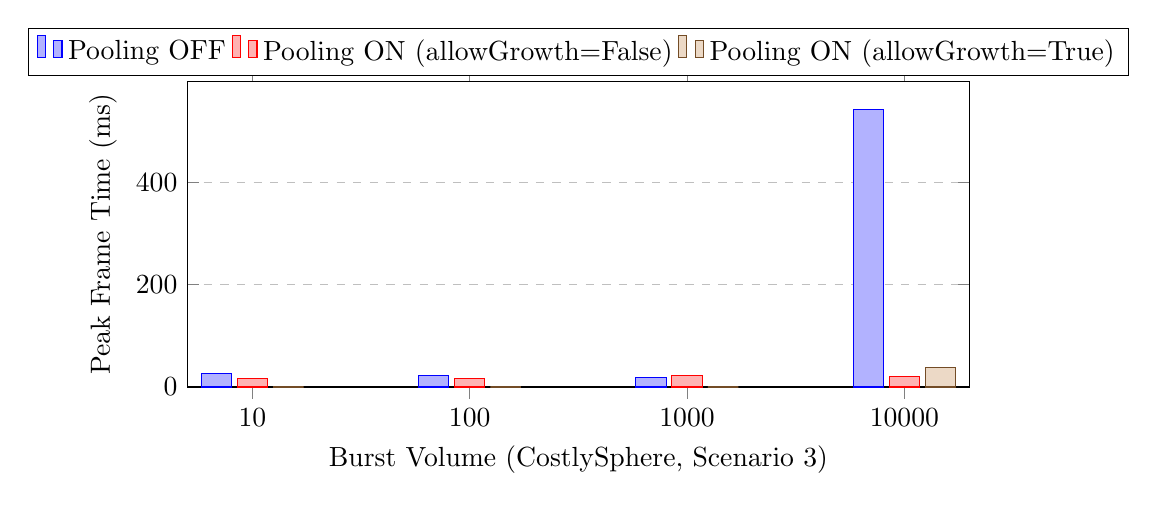
\begin{tikzpicture}
        \begin{axis}[
            ybar,
            bar width=11pt,
            width=0.95\linewidth,
            height=0.45\linewidth,
            ymin=0,
            ylabel={Peak Frame Time (ms)},
            xlabel={Burst Volume (CostlySphere, Scenario 3)},
            symbolic x coords={10,100,1000,10000},
            xtick=data,
            legend style={at={(0.5,1.02)},anchor=south,legend columns=3},
            ymajorgrids=true,
            grid style=dashed
        ]
            \addplot coordinates {(10,25.66) (100,21.66) (1000,19.02) (10000,541.40)};
            \addplot coordinates {(10,17.04) (100,17.10) (1000,22.34) (10000,20.82)};
            \addplot coordinates {(10,0) (100,0) (1000,0) (10000,38.26)};
            \legend{Pooling OFF,Pooling ON (allowGrowth=False),Pooling ON (allowGrowth=True)}
        \end{axis}
    \end{tikzpicture}
    \caption{Scenario 3 burst-latency comparison at \(60\,\mathrm{Hz}\). The native path exhibits a half-second-class stall at \(10{,}000\) entities (\(541.40\,\mathrm{ms}\), Run \#27), while the fully served growth-enabled pooled path remains bounded at \(38.26\,\mathrm{ms}\) (Run \#29), exposing the latency-control effect of the optimized \(O(1)\) pool architecture under volumetric stress.}
    \label{fig:burst_latency_comparison}
\end{figure}

\begin{figure}[htbp]
    \centering
    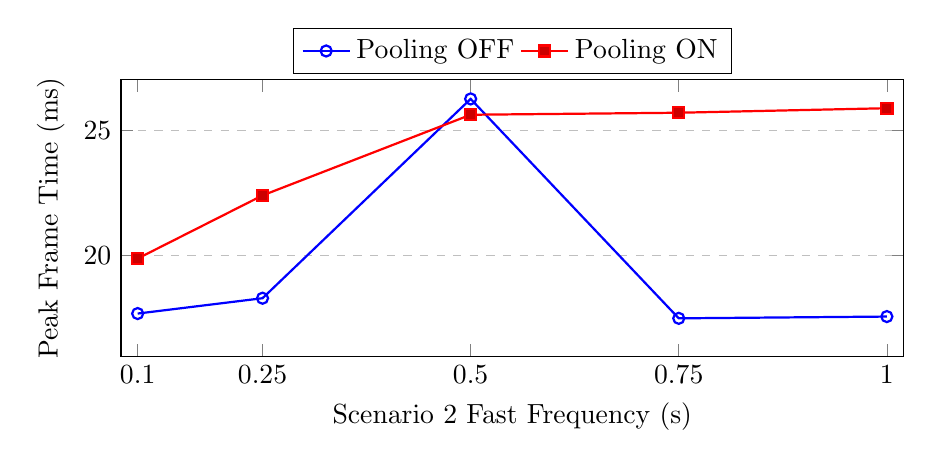
\begin{tikzpicture}
        \begin{axis}[
            width=0.95\linewidth,
            height=0.42\linewidth,
            xmin=0.08, xmax=1.02,
            ymin=16, ymax=27,
            xlabel={Scenario 2 Fast Frequency (s)},
            ylabel={Peak Frame Time (ms)},
            xtick={0.10,0.25,0.50,0.75,1.00},
            ymajorgrids=true,
            grid style=dashed,
            legend style={at={(0.5,1.02)},anchor=south,legend columns=2}
        ]
            \addplot+[mark=o, thick] coordinates {(0.10,17.70) (0.25,18.31) (0.50,26.24) (0.75,17.51) (1.00,17.58)};
            \addplot+[mark=square*, thick] coordinates {(0.10,19.89) (0.25,22.40) (0.50,25.61) (0.75,25.69) (1.00,25.87)};
            \legend{Pooling OFF, Pooling ON}
        \end{axis}
    \end{tikzpicture}
    \caption{Scenario 2 peak-frame-time scaling across fast-frequency tiers. The pooled path sustains higher latency in \(0.75\text{--}1.00\,\mathrm{s}\) tiers, indicating non-trivial runtime management overhead despite similar mean FPS.}
    \label{fig:scenario2_peak_scaling}
\end{figure}

\begin{figure}[htbp]
    \centering
    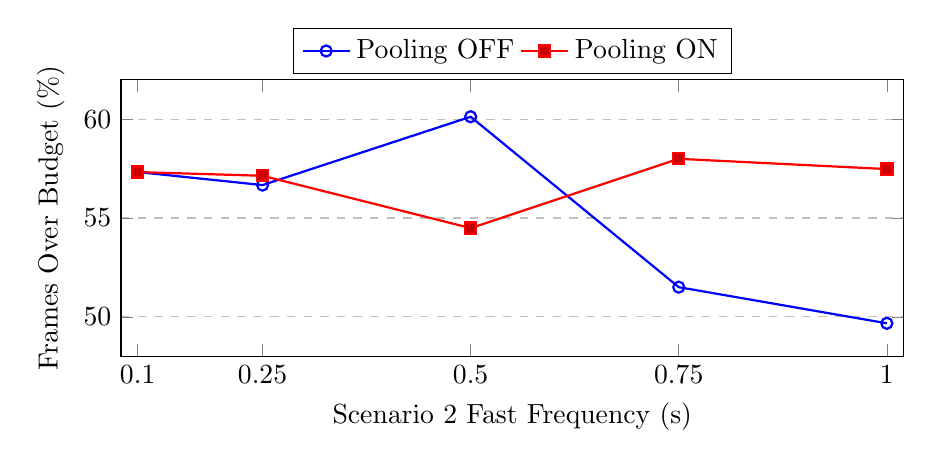
\begin{tikzpicture}
        \begin{axis}[
            width=0.95\linewidth,
            height=0.42\linewidth,
            xmin=0.08, xmax=1.02,
            ymin=48, ymax=62,
            xlabel={Scenario 2 Fast Frequency (s)},
            ylabel={Frames Over Budget (\%)},
            xtick={0.10,0.25,0.50,0.75,1.00},
            ymajorgrids=true,
            grid style=dashed,
            legend style={at={(0.5,1.02)},anchor=south,legend columns=2}
        ]
            \addplot+[mark=o, thick] coordinates {(0.10,57.33) (0.25,56.67) (0.50,60.13) (0.75,51.50) (1.00,49.67)};
            \addplot+[mark=square*, thick] coordinates {(0.10,57.33) (0.25,57.14) (0.50,54.49) (0.75,58.00) (1.00,57.48)};
            \legend{Pooling OFF, Pooling ON}
        \end{axis}
    \end{tikzpicture}
    \caption{Scenario 2 frame-budget violation ratio under \(60\,\mathrm{Hz}\) lock. Pairwise trends show that mean FPS parity does not guarantee better budget adherence.}
    \label{fig:scenario2_budget_violations}
\end{figure}

\begin{figure}[htbp]
    \centering
    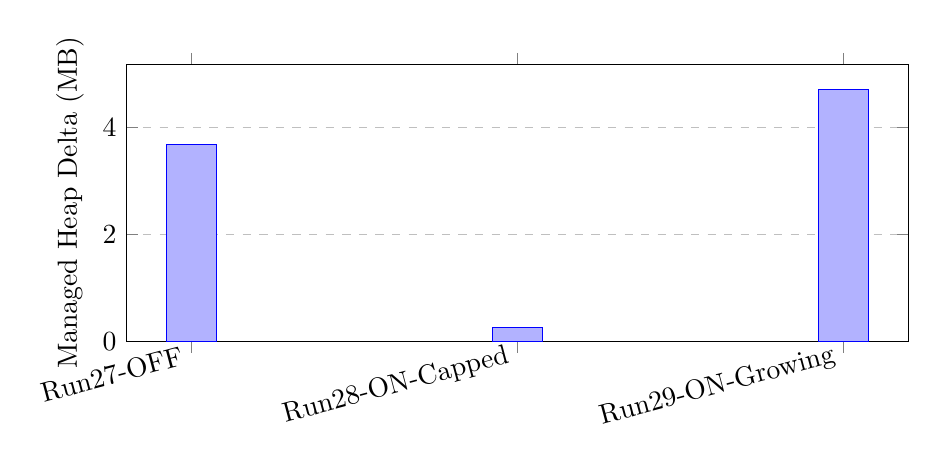
\begin{tikzpicture}
        \begin{axis}[
            ybar,
            bar width=18pt,
            width=0.95\linewidth,
            height=0.42\linewidth,
            ymin=0,
            ylabel={Managed Heap Delta (MB)},
            symbolic x coords={Run27-OFF,Run28-ON-Capped,Run29-ON-Growing},
            xtick=data,
            xticklabel style={rotate=15,anchor=east},
            ymajorgrids=true,
            grid style=dashed
        ]
            \addplot coordinates {(Run27-OFF,3.68) (Run28-ON-Capped,0.26) (Run29-ON-Growing,4.70)};
        \end{axis}
    \end{tikzpicture}
    \caption{Managed-heap deltas at the \(10{,}000\)-burst milestone (CostlySphere). Capped pooling suppresses allocations by rejecting \(90\%\) of requests, whereas growth mode serves the full workload with elevated memory footprint.}
    \label{fig:run27_29_heap}
\end{figure}

\begin{figure}[htbp]
    \centering
    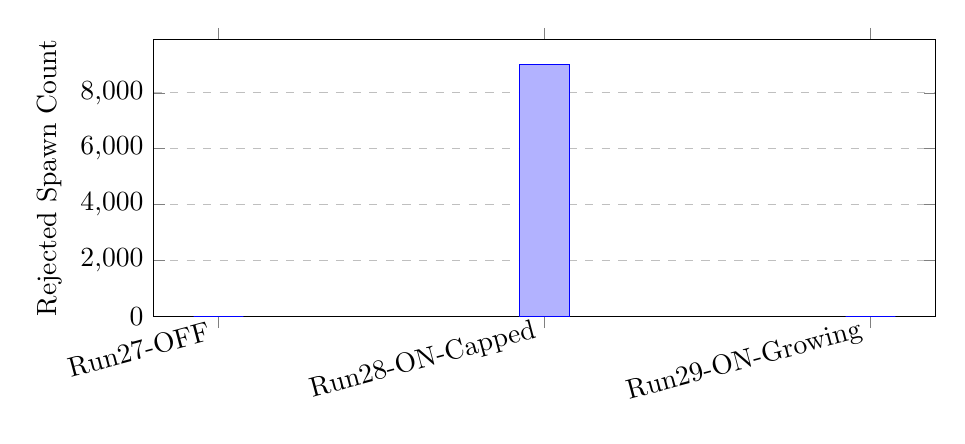
\begin{tikzpicture}
        \begin{axis}[
            ybar,
            bar width=18pt,
            width=0.95\linewidth,
            height=0.42\linewidth,
            ymin=0,
            ylabel={Rejected Spawn Count},
            symbolic x coords={Run27-OFF,Run28-ON-Capped,Run29-ON-Growing},
            xtick=data,
            xticklabel style={rotate=15,anchor=east},
            ymajorgrids=true,
            grid style=dashed
        ]
            \addplot coordinates {(Run27-OFF,0) (Run28-ON-Capped,9000) (Run29-ON-Growing,0)};
        \end{axis}
    \end{tikzpicture}
    \caption{Workload-validity diagnostic for \(10{,}000\)-burst comparison. Run \#28 rejects \(9000\) requests, demonstrating why rejection-aware interpretation is mandatory for fair A/B claims.}
    \label{fig:run27_29_rejections}
\end{figure}

\section{Discussion and Performance Analysis}

\subsection{The Volumetric Burst Latency vs.\ Rejection Trade-off}

The decisive stress point of the benchmark is the \(10{,}000\)-entity burst in Scenario 3 (\texttt{CostlySphere}), where latency behavior diverges sharply across lifecycle policies. As reported in Table~\ref{tab:burst_stress} and visualized in Figure~\ref{fig:burst_latency_comparison}, the native execution path (Run \#27, Pooling OFF) reaches a catastrophic \(541.40\,\mathrm{ms}\) peak frame excursion. Architecturally, this aligns with worst-case engine behavior: high-volume \texttt{Instantiate}/\texttt{Destroy} pressure triggers repeated managed-to-native marshaling plus large-scale transform-hierarchy mutations on the C++ side, which are synchronized on the main thread and therefore directly converted into frame-budget violations.

The apparent superiority of Run \#28 (Pooling ON, \texttt{allowGrowth=False}) must be interpreted as a workload-equivalence illusion rather than a true algorithmic win. While peak latency drops to \(20.82\,\mathrm{ms}\), the run serves only \(1000\) of \(10{,}000\) requests and rejects \(9000\) (\(90\%\)); thus, it does not execute the same computational workload as Run \#27. This is explicitly visible in Table~\ref{tab:burst_stress} and Figure~\ref{fig:run27_29_rejections}. By contrast, Run \#29 (Pooling ON, \texttt{allowGrowth=True}) serves all \(10{,}000\) requests with zero rejection, while bounding the worst-case peak at \(38.26\,\mathrm{ms}\). Although this exceeds the \(16.67\,\mathrm{ms}\) target budget, it avoids a half-second-class stall and therefore represents a controlled latency envelope under full-load equivalence, at the cost of measured reserved-memory expansion (\(+34.48\,\mathrm{MB}\)) and larger inactive residency.

\subsection{Steady-State Management Overhead and Hardware Cache Dynamics}

Scenario 2 reveals a counter-intuitive steady-state phenomenon: pooled execution does not always minimize peak latency under lighter concurrent streams. As shown in Table~\ref{tab:frequency_scaling} and Figure~\ref{fig:scenario2_peak_scaling}, the ON path records \(25.69\,\mathrm{ms}\) and \(25.87\,\mathrm{ms}\) peaks at \(0.75\,\mathrm{s}\) and \(1.00\,\mathrm{s}\), respectively, compared with \(17.51\,\mathrm{ms}\) and \(17.58\,\mathrm{ms}\) in the OFF path. This indicates that in low-entropy regimes, the management overhead of maintaining a large memory-resident inactive set (and associated lifecycle bookkeeping) can dominate the marginal cost of transient primitive allocation.

From a systems perspective on Apple M3 unified memory, this behavior is consistent with cache-locality trade-offs: when instantaneous spawn pressure is low, maintaining and touching a larger pooled state can increase effective cache-miss sensitivity and metadata traversal overhead relative to short-lived native allocations of simple geometry. The outcome is not a contradiction of pooling theory, but a boundary condition: \(O(1)\) access complexity constrains asymptotic retrieval cost, yet constant factors (engine callback overhead, component toggling paths, memory locality) still determine practical latency in light-load tiers.

\subsection{Memory Residency and Garbage Collection Isolation}

The measurement pipeline (\texttt{PrepareEnvironmentBetweenTests}, \texttt{ForceGcAndCooldown}, and heap-stability gating before capture) materially improves phase isolation by forcing garbage collection and introducing a stabilization window before timing begins. This design reduces cross-run contamination and enables more interpretable deltas for \texttt{ManagedHeapDeltaMb} and GC counters. The resulting trends in Table~\ref{tab:burst_stress} and Figure~\ref{fig:run27_29_heap} show the expected policy-dependent memory behavior: capped pooling can suppress runtime allocation churn by reusing pre-resident objects, whereas growth-enabled full-service runs trade temporal resilience for higher memory residency under volumetric demand.

Empirically, the isolation strategy makes the policy trade-off explicit. In the capped \(10{,}000\)-burst path (Run \#28), lower managed-heap delta (\(0.26\,\mathrm{MB}\)) coincides with hard rejection of excess work, while growth mode (Run \#29) reports higher managed-heap movement (\(4.70\,\mathrm{MB}\)) and reserved-memory growth due to full workload admission. Therefore, memory residency should be interpreted as a deliberate control variable, not an artifact: strict cutoff minimizes churn but compromises workload equivalence, while growth mode preserves semantic completeness and bounded latency at the expense of additional memory headroom.

\section{Conclusion}

This report presented an end-to-end empirical evaluation of a high-performance object pooling architecture under bounded frame budgets, implemented through \texttt{PoolManager}, \texttt{ObjectPool<T>}, and deterministic orchestration in \texttt{BatchExperimentRunner}. The system design emphasized \(O(1)\)-oriented retrieval/return semantics, controlled growth policies, rejection-aware accounting, and engine-side lifecycle optimizations that reduce avoidable runtime topology churn. To ensure methodological validity, the benchmark pipeline enforced strict run isolation, explicit garbage-collection stabilization, and fixed-\(60\,\mathrm{Hz}\) frame-budget control.

The results demonstrate that pooling is most valuable as a temporal-stability mechanism in volumetric stress conditions, not as a universal latency minimizer for all workload regimes. Under equivalent \(10{,}000\)-burst demand, growth-enabled pooling bounded worst-case latency to \(38.26\,\mathrm{ms}\), avoiding the native \(541.40\,\mathrm{ms}\) stall, while incurring increased memory residency. Conversely, capped pooling can appear artificially superior when it rejects substantial workload, reinforcing that rejected-spawn accounting is mandatory for fair A/B interpretation. In lighter steady-state tiers, pooled execution may exhibit higher peak latency due to management overhead and locality effects, indicating that constant-time asymptotic complexity alone does not eliminate constant-factor costs.

Overall, the study establishes a practical decision framework: use pooling with explicit policy control, fairness diagnostics, and memory headroom planning when latency collapse under burst pressure is unacceptable; avoid unqualified ``pooling is always faster'' claims in low-entropy scenarios without workload-equivalence checks. Future extensions should include adaptive runtime policy switching (cutoff vs.\ growth), per-object-class pool sizing heuristics, and cross-platform validation to quantify hardware-specific cache and memory effects beyond the Apple M3 baseline.

\end{document}
